% IF YOU CAN SEE THIS GO CONTRIBUTE >:(

\documentclass[letterpaper, 8pt]{extarticle}
\usepackage{amssymb,amsmath,amsthm,amsfonts}
\usepackage{multicol,multirow}
\usepackage{calc}
\usepackage{ifthen}
\usepackage[landscape]{geometry}
\usepackage[colorlinks=true,citecolor=blue,linkcolor=blue]{hyperref}

\usepackage{booktabs}
\usepackage{ulem}
\usepackage{enumitem}
\usepackage{tabulary}
\usepackage{graphicx}
\usepackage{siunitx}
\usepackage{tikz}
\usepackage{derivative}
\usepackage{svg}
\usepackage{listings}
\usepackage{setspace}
\usepackage{listings}
\usepackage{xcolor}
\usepackage{courier}
\usepackage{syntax}
\usepackage{mathpartir}

% minimal line spacing
\setstretch{0.1}

% set borders (experimentally determined to minimize cutoff and maximize space on school printers)
\geometry{top=.25in,left=.25in,right=.25in,bottom=.35in}

% make figures work better in multicol
\newenvironment{Figure}
{\par\medskip\noindent\minipage}
{\endminipage\par\medskip}

\pagestyle{empty} % clear page

% rewrite section commands to be smaller
\makeatletter
\renewcommand{\section}{\@startsection{section}{1}{0mm}%
                                {-1explus -.5ex minus -.2ex}%
                                {0.5ex plus .2ex}%x
                                {\normalfont\normalsize\bfseries}}
\renewcommand{\subsection}{\@startsection{subsection}{2}{0mm}%
                                {-1explus -.5ex minus -.2ex}%
                                {0.5ex plus .2ex}%
                                {\normalfont\small\bfseries}}
\renewcommand{\subsubsection}{\@startsection{subsubsection}{3}{0mm}%
                                {-1ex plus -.5ex minus -.2ex}%
                                {1ex plus .2ex}%
                                {\normalfont\tiny\bfseries}}
\makeatother
\setcounter{secnumdepth}{0} % disable section numbering

% disable indenting
\setlength{\parindent}{0pt}
\setlength{\parskip}{0pt plus 0.5ex}

% Custom siunitx defs
\DeclareSIUnit\noop{\relax}
\NewDocumentCommand\prefixvalue{m}{%
\qty[prefix-mode=extract-exponent,print-unity-mantissa=false]{1}{#1\noop}
}

% Shorthand definitions
\newcommand{\To}{\Rightarrow}
\newcommand{\ttt}{\texttt}

% condense itemize & enumerate
\let\olditemize=\itemize \let\endolditemize=\enditemize \renewenvironment{itemize}{\olditemize \itemsep0em}{\endolditemize}
\let\oldenumerate=\enumerate \let\endoldenumerate=\endenumerate \renewenvironment{enumerate}{\oldenumerate \itemsep0em}{\endoldenumerate}
\setlist[itemize]{noitemsep, topsep=0pt, leftmargin=*}
\setlist[enumerate]{noitemsep, topsep=0pt, leftmargin=*}

\title{3MI3}

\begin{document}
\raggedright
\tiny

% make listings look nicer
\lstset{
    tabsize = 2, %% set tab space width
    showstringspaces = false, %% prevent space marking in strings, string is defined as the text that is generally printed directly to the console
    basicstyle = \tiny\ttfamily, %% set listing font and size
    breaklines = true, %% enable line breaking
    numberstyle = \tiny,
    postbreak = \mbox{\textcolor{red}{\(\hookrightarrow\)}\space}
}

\begin{center}
    {\textbf{3MI3 Final -- Year of the Rabbit Edition}} \\
\end{center}
% set column spacing rules
\setlength{\premulticols}{1pt}
\setlength{\postmulticols}{1pt}
\setlength{\multicolsep}{1pt}
\setlength{\columnsep}{2pt}
\begin{multicols*}{5}
    \section{Syntax}
    How a programming language ``looks''.
    Often a string, but can be a picture (Monet), or a grid of cells (Excel).
    \subsection{BNF}
    Formal specification of string-based syntaxes.
    \begin{grammar}
        <e> ::= x
        \alt \(\lambda x <e>\)
        \alt <e> <e>
        \alt (<e>)
    \end{grammar}

    \section{Dynamic Semantics}
    % Small-step semantics
    % -> Lambda calculus - Call-by-name vs Call-by-value
    % domain-specific languages
    % shallow vs deep vs tagless embeddings

    \subsection{Evaluation Strategies}

    Can't evaluate anything under a lambda in both of the below strategies.

    \textbf{Call by name} --
    Can't evaluate anything that isn't an outermost term.
    % idk put the rules or an example here

    % TODO: if we run out of space delete this and replace it with an explanation
    \(\inferrule{e_1 \to e_1'}{e_1 e_2 \to e_1' e_2}\)
    \(\inferrule{ }{(\lambda x.e_1)e_2 \to e_1[e_2/x]}\)
    \(\inferrule{ }{\operatorname{fst}(e_2, e_2) \to e_2}\)
    \(\inferrule{ }{\operatorname{snd}(e_1, e_2) \to e_2}\)
    \(\inferrule{e_1 \to e_1'}{\operatorname{and} e_1 e_2 \to \operatorname{and} e_1' e_2}\)
    \(\inferrule{ }{\operatorname{and}\operatorname{true} e_2 \to e_2}\)
    \(\inferrule{ }{\operatorname{and}\operatorname{false} e_2 \to \operatorname{false}}\)
    \(\inferrule{e_1 \to e_1'}{\operatorname{if} e_1 \operatorname{then} e_2 \operatorname{else} e_3 \to \operatorname{if} e_1' \operatorname{then} e_2 \operatorname{else} e_3}\)
    \(\inferrule{ }{\operatorname{if}\operatorname{true}\operatorname{then} e_2 \operatorname{else} e_3 \to e_2}\)
    \(\inferrule{ }{\operatorname{if}\operatorname{false}\operatorname{then} e_2 \operatorname{else} e_3 \to e_3}\)
    \(\inferrule{ }{\operatorname{let} x = e_1 \operatorname{in} e_2 \to e_2[e_1/x]}\)

    \textbf{Call by Value} --
    Reduce arguments first

    \(\inferrule{e_1 \to e_1'}{e_1 e_2 \to e_1' e_2}\)
    \(\inferrule{e_2 \to e_2'}{v_1 e_2 \to v_1 e_2'}\)
    \(\inferrule{ }{(\lambda x.e_1) v_2 \to e_1[v_2/x]}\)
    \(\inferrule{e_1 \to e_1'}{(e_1, e_2) \to (e_1', e_2)}\)
    \(\inferrule{e_2 \to e_2'}{(v_1, e_2) \to (v_1, e_2')}\)
    \(\inferrule{ }{\operatorname{fst} (v_1, v_2) \to v_1}\)
    \(\inferrule{ }{\operatorname{snd} (v_1, v_2) \to v_2}\)
    \(\inferrule{e_1 \to e_1'}{\operatorname{and} e_1 e_2 \to \operatorname{and} e_1' e_2}\)
    \(\inferrule{ }{\operatorname{and}\operatorname{true} e_2 \to e_2}\)
    \(\inferrule{ }{\operatorname{and}\operatorname{false} e_2 \to \operatorname{false}}\)
    \(\inferrule{e_1 \to e_1'}{\operatorname{if} e_1 \operatorname{then} e_2 \operatorname{else} e_3 \to \operatorname{if} e_1' \operatorname{then} e_2 \operatorname{else} e_3}\)
    \(\inferrule{ }{\operatorname{if}\operatorname{true}\operatorname{then} e_2 \operatorname{else} e_3 \to e_2}\)
    \(\inferrule{ }{\operatorname{if}\operatorname{false}\operatorname{then} e_2 \operatorname{else} e_3 \to e_3}\)
    \(\inferrule{e_1 \to e_1'}{\operatorname{let} x = e_1 \operatorname{in} e_2 \to \operatorname{let} x = e_1' \operatorname{in} e_2}\)
    \(\inferrule{ }{\operatorname{let} x = v_1 \operatorname{in} e_2 \to e_2[v_1/x]}\)

    \subsection{Church Encodings}
    \subsubsection{Pairs}
    pair = $\lambda x.\lambda y.\lambda z.z\,x\,y$\\
    fst = $\lambda p.p (\lambda x.\lambda y.x)$\\
    snd = $\lambda p.p (\lambda x.\lambda y.y)$

    \subsubsection{Lists}
    nil = $\lambda c.\lambda n.n$\\
    cons = $\lambda h.\lambda t.\lambda c.\lambda n.c\,h\,(t\,c\,n)$

    % credit to milenb17#9439 on Discord
    \subsubsection{Trees}
    leaf = \(\lambda x.\lambda b.\lambda l.l ,x\)\\
    branch = \(\lambda x.\lambda y.\lambda b.\lambda l. ,b ,(x, l, b) ,(y, l, b)\)

    \subsection{Domain Specific Languages (DSLs)}
    \subsubsection{Shallow}
    Implement the DSL as functions.
    Ex. for pic DSL, stuff is given as functions.
    Easy to add new functions,
    but can suck if you want to extend to more interpretations since you can't reuse functions.
    \subsubsection{Deep}
    Datatype to represent syntax.
    Can easily write new interpretation functions.
    But annoying to add new operations because all interpretations need to be extended.
    \subsubsection{Tagless}
    Best of shallow and deep.
    The language is the interpretation.
    If we want to add a new operation we can easily add a new class that extends the original.
    To create a new interpretation just create an instance of the class.

    \section{Static Semantics (Typing)}
    % types
    % Progress rule (always be able to make a step towards the value)
    % (for every well-typed program, either I can make a step, or e is a value)
    % Preservation rule (if a term is well-typed, and we evaluate it once under
    % single-step operational semantics, the resulting term is also well typed.)

    \subsection{Progress}
    \subsection{Preservation}


    \subsection{Context}
    % context list and how it works
    % unification (????? idk i didnt pay attention to this section)
    % u jus like me fr
    \subsection{Unification}
    \subsubsection{Unification Algorithm}
    % Note: screenshotted from tb p327, transcribe if you want
    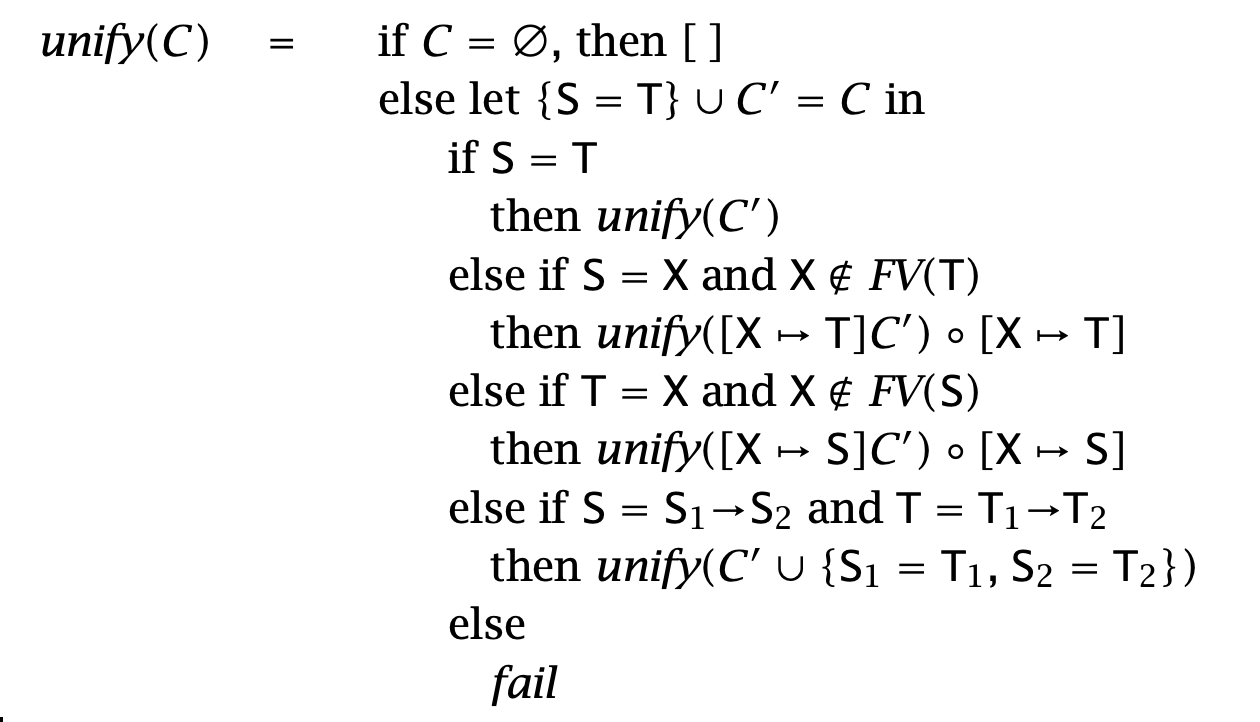
\includegraphics[width=\linewidth]{unification-algorithm.png}

    % featherweight java (wtf?)

    % subtyping
    \subsection{Subtyping}
    T-Sub: \(\frac{\Gamma \vdash t : S \quad S <: T}{\Gamma \vdash t : T}\)\\
    S-Refl: \(S <: S\)\\
    S-Trans: \(\frac{S<: U \quad U<:T}{S<:T}\)\\
    S-RcdWidth: \(\{ l_{i}: T_{i}^{i \in  1..n +k} \} <: \{ l_{i}: T_{i}^{i \in  1..n} \}\)\\
    S-RcdDepth: \(\frac{\text{for each } i \quad S_{i} <: T_{i}}{\{ l_{i}: S_{i}^{i \in  1..n } \} <: \{ l_{i}: T_{i}^{i \in  1..n} \}}\)\\
    S-RcdPerm: \(\frac{\{k_{j} :S_{j}^{j \in 1..n}\} \text{ is perm. of } \{l_{i}:T_{i}^{i \in 1..n} \}}{\{k_{j}:S_{j}^{j \in 1..n} \} <: \{l_{i}: T_{I}^{i \in 1..n} \}}\)\\
    S-Arrow: \(\frac{T_{1} <: S_{1} \quad S_{2} <: T_{2}}{S_{1} \to S_{2} <: T_{1} \to T_{2}}\)\\
    This S-Arrow subtype relation is \textbf{contravariant} in the left-hand sides of arrows, and
    \textbf{covariant} in the right-hand sides of arrows.
    The intuition is that if we have a function \(S_1 \to S_2\),
    then it will accept any subtype of \(S_1\) as input,
    and the result \(S_2\) can be viewed as belonging to any supertype of \(S_2\).\\
    S-Top: \(S<: \text{Top}\), where \(\text{Top}\) is a new type constant that is a supertype of every type.

    \section{Q\&A}

    \subsection{Q1 Practice Answer}

    % CBN Example
    %((λx.λy.y y)((λw.w w)(λw.w w)))(λw.w)  
    %(λy.y y) (λw.w) - λx is called, all x’s replaced w/ (λw.w w)(λw.w w) 
    %(λw.w) (λw.w) - λy is called, all y’s replaced w/ (λw.w)
    %(λw.w) - λw is called, all w’s replaced w/ (λw.w)
    \subsubsection{CBN}
    \begin{align*}
         & ((\lambda x.\lambda y.y y)((\lambda w.w w)(\lambda w.w w)))(\lambda w.w)      \\
         & \textrm{//\(\lambda x\) is called, all \(x\)'s replaced}                      \\
         & (\lambda y.y y) (\lambda w.w)                                                 \\
         & \textrm{//\(\lambda y\) is called, all \(y\)'s replaced w/ \((\lambda w.w)\)} \\
         & (\lambda w.w) (\lambda w.w)                                                   \\
         & \textrm{//\(\lambda w\) is caled, all \(w\)'s replaced w/ \((\lambda w.w)\)}  \\
         & (\lambda w.w)
    \end{align*}

    %CBV Example
    % (λx.λy.y y)((λw.w w)(λw.w w))(λw.w) 
    %(λx.λy.y y)((λw.w w)(λw.w w))(λw.w) - λw is called, all w’s replaced w/ (λw.w w)
    % Does not terminate, infinite loop of (λw.w w)(λw.w w)
    \subsubsection{CBV}
    \begin{align*}
         & (\lambda x.\lambda y.y y)((\lambda w.w w)(\lambda w.w w))(\lambda w.w) \\
         & (\lambda x.\lambda y.y y)((\lambda w.w w)(\lambda w.w w))(\lambda w.w) \\
         & \textrm{//infinite loop}
    \end{align*}

\end{multicols*}

\end{document}
